\chapter{Results \textit{\&} Discussion}

\section{Visualizing RetNet}

\begin{figure}
	\centering
	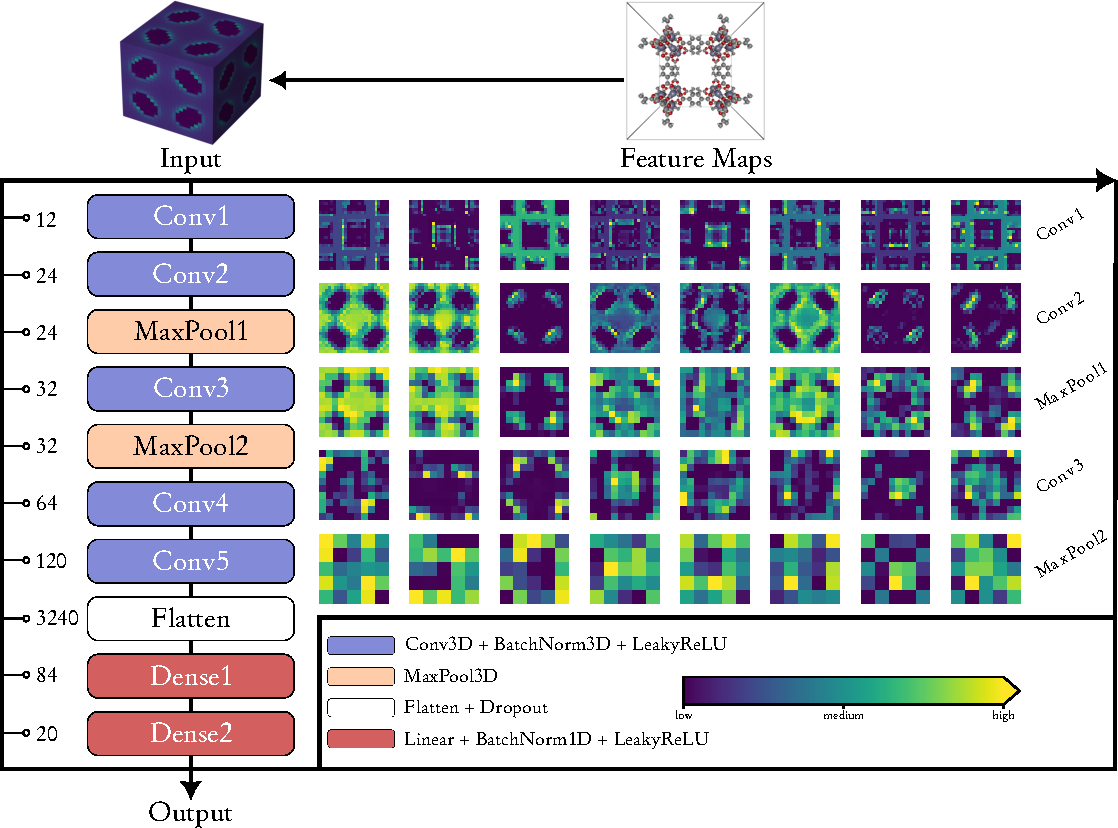
\includegraphics[width=\textwidth]{fig/forward_pass.pdf}
	\caption{Foo}
	\label{fig:retnet}
\end{figure}

\begin{figure}
	\centering
	\begin{subfigure}[b]{0.49\textwidth}
		\centering
		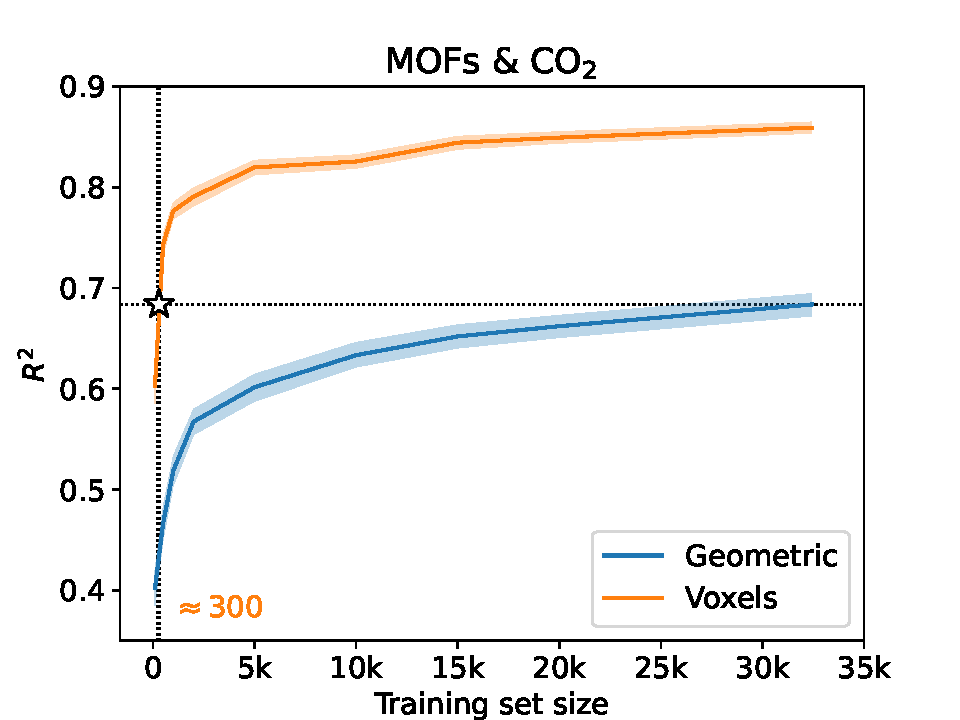
\includegraphics[width=\textwidth]{fig/learning_curves_mofs.pdf}
		\caption{Learning curves for \glspl{mof} \textit{\&} \ch{CO2}.}
		\label{fig:learning_curves_mofs}
	\end{subfigure}
	\begin{subfigure}[b]{0.49\textwidth}
		\centering
		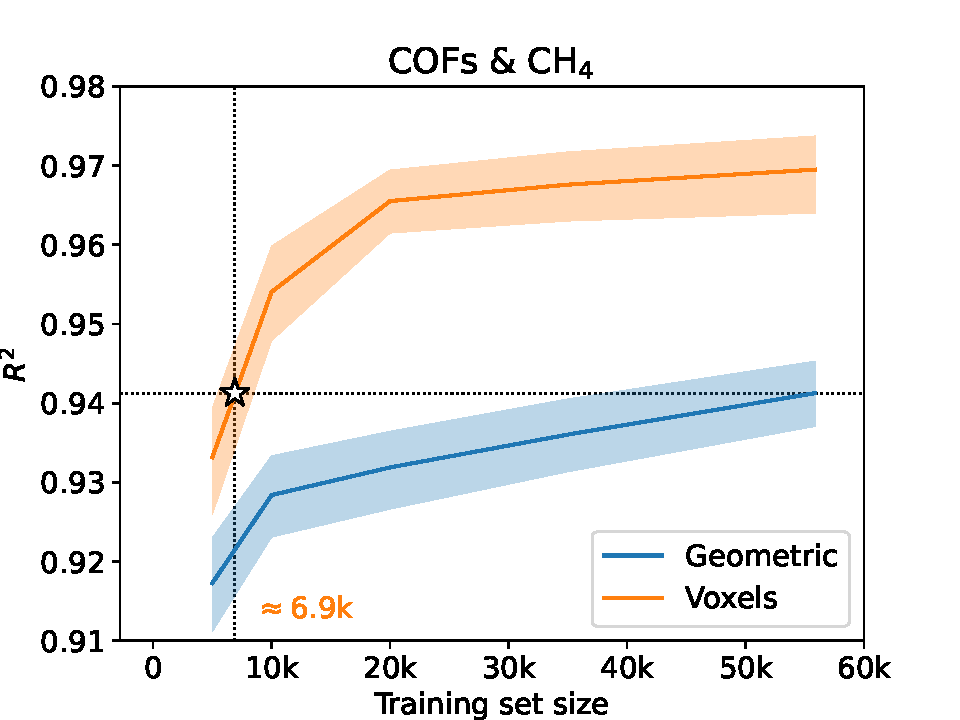
\includegraphics[width=\textwidth]{fig/learning_curves_cofs.pdf}
		\caption{Learning curves for \glspl{cof} \textit{\&} \ch{CH4}.}
		\label{fig:learning_curves_cofs}
	\end{subfigure}
	\caption{Performance ($R^2$ score) on test set as function of the training
	set size for conventional and \gls{cnn} models. Shaded areas correspond to
	the \SI{95}{\percent} \gls{ci}\index{Confidence interval}. The
	$x$-coordinate of the white star denotes the trainig set size where the
	\gls{cnn} model reaches the performance of the conventional one, the
	$y$-coordinate. ``Geometric'' stands for geometric descriptors, while
	``Voxels'' stands for energy voxels.}
	\label{fig:learning_curves}
\end{figure}

\begin{equation}
	2 = 3
\end{equation}
